\documentclass{ximera}

%\usepackage{todonotes}

\newcommand{\todo}{}

\usepackage{esint} % for \oiint
\ifxake%%https://math.meta.stackexchange.com/questions/9973/how-do-you-render-a-closed-surface-double-integral
\renewcommand{\oiint}{{\large\bigcirc}\kern-1.56em\iint}
\fi


\graphicspath{
  {./}
  {ximeraTutorial/}
  {basicPhilosophy/}
  {functionsOfSeveralVariables/}
  {normalVectors/}
  {lagrangeMultipliers/}
  {vectorFields/}
  {greensTheorem/}
  {shapeOfThingsToCome/}
  {dotProducts/}
  {partialDerivativesAndTheGradientVector/}
  {../productAndQuotientRules/exercises/}
  {../normalVectors/exercisesParametricPlots/}
  {../continuityOfFunctionsOfSeveralVariables/exercises/}
  {../partialDerivativesAndTheGradientVector/exercises/}
  {../directionalDerivativeAndChainRule/exercises/}
  {../commonCoordinates/exercisesCylindricalCoordinates/}
  {../commonCoordinates/exercisesSphericalCoordinates/}
  {../greensTheorem/exercisesCurlAndLineIntegrals/}
  {../greensTheorem/exercisesDivergenceAndLineIntegrals/}
  {../shapeOfThingsToCome/exercisesDivergenceTheorem/}
  {../greensTheorem/}
  {../shapeOfThingsToCome/}
  {../separableDifferentialEquations/exercises/}
  {vectorFields/}
}

\newcommand{\mooculus}{\textsf{\textbf{MOOC}\textnormal{\textsf{ULUS}}}}

\usepackage{tkz-euclide}
\usepackage{tikz}
\usepackage{tikz-cd}
\usetikzlibrary{arrows}
\tikzset{>=stealth,commutative diagrams/.cd,
  arrow style=tikz,diagrams={>=stealth}} %% cool arrow head
\tikzset{shorten <>/.style={ shorten >=#1, shorten <=#1 } } %% allows shorter vectors

\usetikzlibrary{backgrounds} %% for boxes around graphs
\usetikzlibrary{shapes,positioning}  %% Clouds and stars
\usetikzlibrary{matrix} %% for matrix
\usepgfplotslibrary{polar} %% for polar plots
\usepgfplotslibrary{fillbetween} %% to shade area between curves in TikZ
%\usetkzobj{all}
\usepackage[makeroom]{cancel} %% for strike outs
%\usepackage{mathtools} %% for pretty underbrace % Breaks Ximera
%\usepackage{multicol}
\usepackage{pgffor} %% required for integral for loops



%% http://tex.stackexchange.com/questions/66490/drawing-a-tikz-arc-specifying-the-center
%% Draws beach ball
\tikzset{pics/carc/.style args={#1:#2:#3}{code={\draw[pic actions] (#1:#3) arc(#1:#2:#3);}}}



\usepackage{array}
\setlength{\extrarowheight}{+.1cm}
\newdimen\digitwidth
\settowidth\digitwidth{9}
\def\divrule#1#2{
\noalign{\moveright#1\digitwidth
\vbox{\hrule width#2\digitwidth}}}




% \newcommand{\RR}{\mathbb R}
% \newcommand{\R}{\mathbb R}
% \newcommand{\N}{\mathbb N}
% \newcommand{\Z}{\mathbb Z}

\newcommand{\sagemath}{\textsf{SageMath}}


%\renewcommand{\d}{\,d\!}
%\renewcommand{\d}{\mathop{}\!d}
%\newcommand{\dd}[2][]{\frac{\d #1}{\d #2}}
%\newcommand{\pp}[2][]{\frac{\partial #1}{\partial #2}}
% \renewcommand{\l}{\ell}
%\newcommand{\ddx}{\frac{d}{\d x}}

% \newcommand{\zeroOverZero}{\ensuremath{\boldsymbol{\tfrac{0}{0}}}}
%\newcommand{\inftyOverInfty}{\ensuremath{\boldsymbol{\tfrac{\infty}{\infty}}}}
%\newcommand{\zeroOverInfty}{\ensuremath{\boldsymbol{\tfrac{0}{\infty}}}}
%\newcommand{\zeroTimesInfty}{\ensuremath{\small\boldsymbol{0\cdot \infty}}}
%\newcommand{\inftyMinusInfty}{\ensuremath{\small\boldsymbol{\infty - \infty}}}
%\newcommand{\oneToInfty}{\ensuremath{\boldsymbol{1^\infty}}}
%\newcommand{\zeroToZero}{\ensuremath{\boldsymbol{0^0}}}
%\newcommand{\inftyToZero}{\ensuremath{\boldsymbol{\infty^0}}}



% \newcommand{\numOverZero}{\ensuremath{\boldsymbol{\tfrac{\#}{0}}}}
% \newcommand{\dfn}{\textbf}
% \newcommand{\unit}{\,\mathrm}
% \newcommand{\unit}{\mathop{}\!\mathrm}
% \newcommand{\eval}[1]{\bigg[ #1 \bigg]}
% \newcommand{\seq}[1]{\left( #1 \right)}
% \renewcommand{\epsilon}{\varepsilon}
% \renewcommand{\phi}{\varphi}


% \renewcommand{\iff}{\Leftrightarrow}

% \DeclareMathOperator{\arccot}{arccot}
% \DeclareMathOperator{\arcsec}{arcsec}
% \DeclareMathOperator{\arccsc}{arccsc}
% \DeclareMathOperator{\si}{Si}
% \DeclareMathOperator{\scal}{scal}
% \DeclareMathOperator{\sign}{sign}


%% \newcommand{\tightoverset}[2]{% for arrow vec
%%   \mathop{#2}\limits^{\vbox to -.5ex{\kern-0.75ex\hbox{$#1$}\vss}}}
% \newcommand{\arrowvec}[1]{{\overset{\rightharpoonup}{#1}}}
% \renewcommand{\vec}[1]{\arrowvec{\mathbf{#1}}}
% \renewcommand{\vec}[1]{{\overset{\boldsymbol{\rightharpoonup}}{\mathbf{#1}}}}

% \newcommand{\point}[1]{\left(#1\right)} %this allows \vector{ to be changed to \vector{ with a quick find and replace
% \newcommand{\pt}[1]{\mathbf{#1}} %this allows \vec{ to be changed to \vec{ with a quick find and replace
% \newcommand{\Lim}[2]{\lim_{\point{#1} \to \point{#2}}} %Bart, I changed this to point since I want to use it.  It runs through both of the exercise and exerciseE files in limits section, which is why it was in each document to start with.

% \DeclareMathOperator{\proj}{\mathbf{proj}}
% \newcommand{\veci}{{\boldsymbol{\hat{\imath}}}}
% \newcommand{\vecj}{{\boldsymbol{\hat{\jmath}}}}
% \newcommand{\veck}{{\boldsymbol{\hat{k}}}}
% \newcommand{\vecl}{\vec{\boldsymbol{\l}}}
% \newcommand{\uvec}[1]{\mathbf{\hat{#1}}}
% \newcommand{\utan}{\mathbf{\hat{t}}}
% \newcommand{\unormal}{\mathbf{\hat{n}}}
% \newcommand{\ubinormal}{\mathbf{\hat{b}}}

% \newcommand{\dotp}{\bullet}
% \newcommand{\cross}{\boldsymbol\times}
% \newcommand{\grad}{\boldsymbol\nabla}
% \newcommand{\divergence}{\grad\dotp}
% \newcommand{\curl}{\grad\cross}
%\DeclareMathOperator{\divergence}{divergence}
%\DeclareMathOperator{\curl}[1]{\grad\cross #1}
% \newcommand{\lto}{\mathop{\longrightarrow\,}\limits}

% \renewcommand{\bar}{\overline}

\colorlet{textColor}{black}
\colorlet{background}{white}
\colorlet{penColor}{blue!50!black} % Color of a curve in a plot
\colorlet{penColor2}{red!50!black}% Color of a curve in a plot
\colorlet{penColor3}{red!50!blue} % Color of a curve in a plot
\colorlet{penColor4}{green!50!black} % Color of a curve in a plot
\colorlet{penColor5}{orange!80!black} % Color of a curve in a plot
\colorlet{penColor6}{yellow!70!black} % Color of a curve in a plot
\colorlet{fill1}{penColor!20} % Color of fill in a plot
\colorlet{fill2}{penColor2!20} % Color of fill in a plot
\colorlet{fillp}{fill1} % Color of positive area
\colorlet{filln}{penColor2!20} % Color of negative area
\colorlet{fill3}{penColor3!20} % Fill
\colorlet{fill4}{penColor4!20} % Fill
\colorlet{fill5}{penColor5!20} % Fill
\colorlet{gridColor}{gray!50} % Color of grid in a plot

\newcommand{\surfaceColor}{violet}
\newcommand{\surfaceColorTwo}{redyellow}
\newcommand{\sliceColor}{greenyellow}




\pgfmathdeclarefunction{gauss}{2}{% gives gaussian
  \pgfmathparse{1/(#2*sqrt(2*pi))*exp(-((x-#1)^2)/(2*#2^2))}%
}


%%%%%%%%%%%%%
%% Vectors
%%%%%%%%%%%%%

%% Simple horiz vectors
\renewcommand{\vector}[1]{\left\langle #1\right\rangle}


%% %% Complex Horiz Vectors with angle brackets
%% \makeatletter
%% \renewcommand{\vector}[2][ , ]{\left\langle%
%%   \def\nextitem{\def\nextitem{#1}}%
%%   \@for \el:=#2\do{\nextitem\el}\right\rangle%
%% }
%% \makeatother

%% %% Vertical Vectors
%% \def\vector#1{\begin{bmatrix}\vecListA#1,,\end{bmatrix}}
%% \def\vecListA#1,{\if,#1,\else #1\cr \expandafter \vecListA \fi}

%%%%%%%%%%%%%
%% End of vectors
%%%%%%%%%%%%%

%\newcommand{\fullwidth}{}
%\newcommand{\normalwidth}{}



%% makes a snazzy t-chart for evaluating functions
%\newenvironment{tchart}{\rowcolors{2}{}{background!90!textColor}\array}{\endarray}

%%This is to help with formatting on future title pages.
\newenvironment{sectionOutcomes}{}{}



%% Flowchart stuff
%\tikzstyle{startstop} = [rectangle, rounded corners, minimum width=3cm, minimum height=1cm,text centered, draw=black]
%\tikzstyle{question} = [rectangle, minimum width=3cm, minimum height=1cm, text centered, draw=black]
%\tikzstyle{decision} = [trapezium, trapezium left angle=70, trapezium right angle=110, minimum width=3cm, minimum height=1cm, text centered, draw=black]
%\tikzstyle{question} = [rectangle, rounded corners, minimum width=3cm, minimum height=1cm,text centered, draw=black]
%\tikzstyle{process} = [rectangle, minimum width=3cm, minimum height=1cm, text centered, draw=black]
%\tikzstyle{decision} = [trapezium, trapezium left angle=70, trapezium right angle=110, minimum width=3cm, minimum height=1cm, text centered, draw=black]


\title{Logarithmic Functions}

\begin{document}

\begin{abstract}
exponents
\end{abstract}
\maketitle






An example of a basic exponential function is $E(t) = 2^t$.  

Its graph looks like







\begin{image}
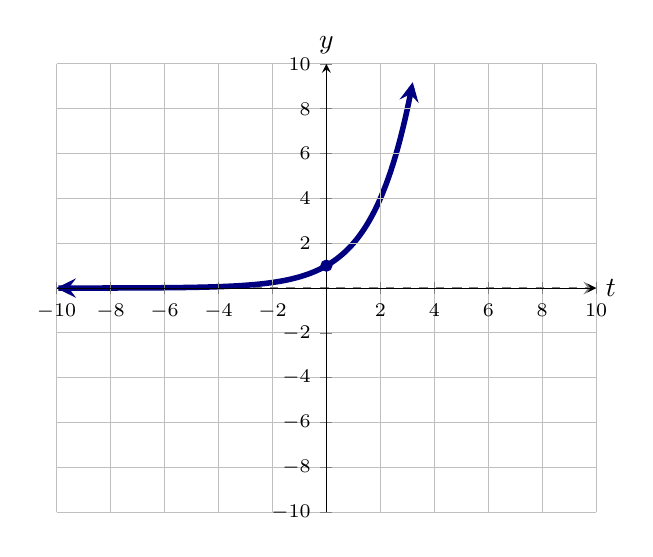
\begin{tikzpicture}
  \begin{axis}[
            domain=-10:10, ymax=10, xmax=10, ymin=-10, xmin=-10,
            axis lines =center, xlabel=$t$, ylabel=$y$, grid = major,
            ytick={-10,-8,-6,-4,-2,2,4,6,8,10},
          	xtick={-10,-8,-6,-4,-2,2,4,6,8,10},
          	ticklabel style={font=\scriptsize},
            every axis y label/.style={at=(current axis.above origin),anchor=south},
            every axis x label/.style={at=(current axis.right of origin),anchor=west},
            axis on top
          ]
          
      		\addplot [line width=1, gray, dashed,samples=200,domain=(-10:10),<->] {0};

          \addplot [line width=2, penColor, smooth,samples=200,domain=(-10:3.2),<->] {2^x};

      		\addplot[color=penColor,fill=penColor,only marks,mark=*] coordinates{(0,1)};

          


  \end{axis}
\end{tikzpicture}
\end{image}






We can evalute this function:
\begin{itemize}
\item $E(0) = 2^0 = 1$
\item $E\left(\frac{1}{2}\right) = 2^{\tfrac{1}{2}} = \sqrt{2}$
\item $E(-1) = 2^{-1} = \frac{1}{2}$
\end{itemize}


When we evaluate a function, we know the domain number and we seek its range partner. In this case, we know $d$ and we seek the pair $(d, 2^d)$, where $2^d$ is the value of the function at $d$.













\section{Reverse}

We can also think in reverse.
\begin{itemize}
\item $E(t) = 4$
\item $E(t) = {\tfrac{1}{4}} $
\item $E(t) = 16 $
\end{itemize}


Here, we know the value of the function.  We seek the domain numbers paired with it. We know $2^d$, we seek the pair $(d, 2^d)$, where $d$ is the solution to the equation.




$\bigstar$ For $E(t) = 2^t$, as long as we give a positive function value, then we can find the associated domain number. \\ 



$\bigstar$ For $E(t) = 2^t$, every positive function value has \textit{exactly one} associated domain number. That is eeriely backwards of the function rule.\\ 



\begin{observation}  \textbf{\textcolor{red!80!black}{Backwards}}

\textbf{Remember:}  Each domain number in a function is paired with exactly one range number.  In other words, a function can have only one value at each domain number. 


We just said a similar sentence for the range numbers of an exponential function.


We just said that each range number for an exponential function is paired with exactly one domain number.

That's not a requirement to be a function.  It is an extra characteristics of exponential functions.



\end{observation}



Thinking of an exponential function in reverse sounds like a new function. It is. We call it a \textbf{\textcolor{purple!85!blue}{logarithmic function}}.








\[
\begin{array}{lcl}
Exponential Function  &     &  Logarithmic Function  \\
domain = (-\infty, \infty)  &  \searrow  &  domain = (0, \infty)  \\
range = (0, \infty)  &  \nearrow  &  range = (-\infty, \infty)  \\
(a, r^a)    &  \longrightarrow  &   (r^a, a)
\end{array}
\]


The logarithm function just reverses the pairs in the exponential function.  If $(a, 2^a)$ is a pair in the exponential function, then $(2^a, a)$ is a pair in the logarithmic function.


Therefore, the domain and range switch. \\






\subsection{Logarithm}

It seems weird to write $(2^a, a)$, even though it is perfectly correct.  

We are used to representing the domain number by a letter, $b$, and then the function value as a formula involving $b$.

We would prefer our pairs in the logarithm function to look like 

\[ (b, expression)  \]


What's the expression? \\





Logarithmic functions come from the study of \textbf{logarithms}, which gets shortened to \textbf{log} for notation purposes.  \\



In our example here, we are working with the base $2$ exponential, $E(t) = 2^t$. So, the reverse is called \textbf{the logarithm base $2$}.  We tack on a subscript $2$ to complete the name of our new function.



\[   \log_2(b)     \]


That pairs in the logarithmic base $2$ function look like 


\[
(b, \log_2(b))
\]


The coordinates of the points on the graph look like



\[
(b, \log_2(b))
\]




$\log_2(b)$ is just the exponent that $2$ needs to equal $b$.





$\blacktriangleright$ \textbf{Remember:} $(b, \log_2(b))$ are the reverse of the exponential pairs : $(a, 2^a)$.  \\

$(b, \log_2(b))$ is also $(2^c, c)$ for some $c$. \\


$\blacktriangleright$  $\log_2(b)$ is the number that you raise $2$ to, to get $b$.  \\

\[   2^{\log_2(b)} = b     \]

We have a logarithmic function for every exponential function.  They are designated by their bases.
















\begin{definition} \textbf{\textcolor{green!50!black}{Logarithm Function base $B$ : $log_B(t)$}}


$\log_B(t)$ is the number you raise $B$ to, to get $t$. \\

$t \in (0, \infty)$. \\

$\log_B(t) \in (-\infty, \infty)$.


\end{definition}






Since all of the pairs are reversed, the graphs switch axes.



The horizontal axis is an asymptote for the basic exponential function. Now, the vertical axis is an asymptote for the basic logarithmic function.


The graph of a basic exponential function has $(0,1)$ as an intercept.  The graph of a basic logarithmic function has $(1,0)$ as an intercept. 


Their graphs are mirror images of each other across the diagonal through quadrants I and III.










\begin{image}
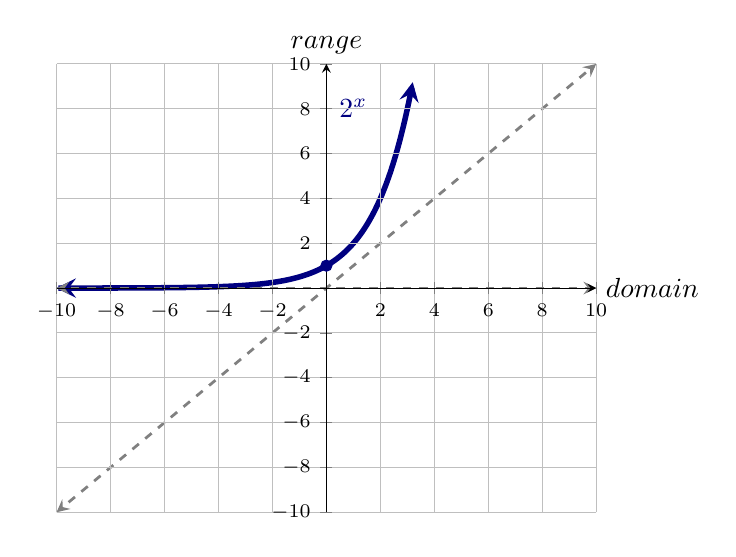
\begin{tikzpicture}
  \begin{axis}[
            domain=-10:10, ymax=10, xmax=10, ymin=-10, xmin=-10,
            axis lines =center, xlabel=$domain$, ylabel=$range$, grid = major,
            ytick={-10,-8,-6,-4,-2,2,4,6,8,10},
          	xtick={-10,-8,-6,-4,-2,2,4,6,8,10},
          	ticklabel style={font=\scriptsize},
            every axis y label/.style={at=(current axis.above origin),anchor=south},
            every axis x label/.style={at=(current axis.right of origin),anchor=west},
            axis on top
          ]
          
      		\addplot [line width=2, penColor, smooth,samples=200,domain=(-10:3.2),<->] {2^x};
      		%\addplot [line width=2, penColor2, smooth,samples=200,domain=(0.003:8),<->] {ln(x)/ln(2)};

          	\addplot [line width=1, gray, dashed,samples=200,domain=(-10:10),<->] {0};
          	%\addplot [line width=1, gray, dashed,samples=200,domain=(-10:10),<->] ({0},{x});
          	\addplot [line width=1, gray, dashed,samples=200,domain=(-10:10),<->] ({x},{x});


      		\addplot[color=penColor,fill=penColor,only marks,mark=*] coordinates{(0,1)};
      		%\addplot[color=penColor2,fill=penColor,only marks,mark=*] coordinates{(1,0)};

      		\node[penColor] at (axis cs:1,8) {$2^x$};
      		%\node[penColor2] at (axis cs:7,1) {$log_2(x)$};





           

  \end{axis}
\end{tikzpicture}
\end{image}













\begin{image}
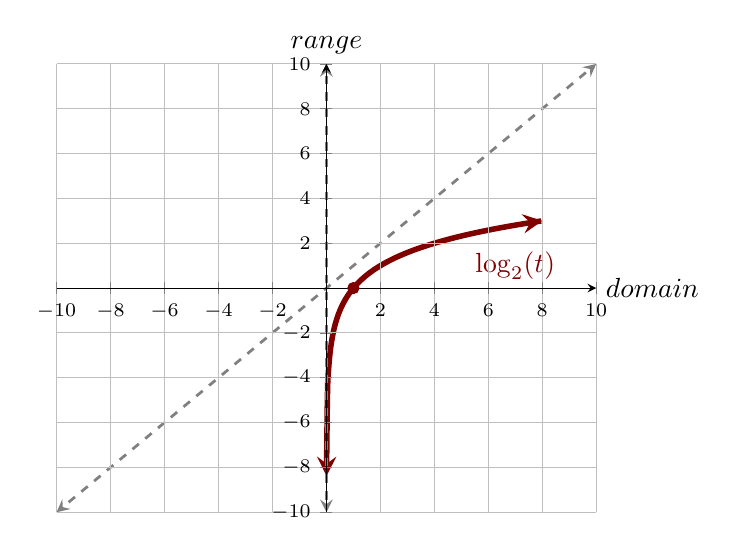
\begin{tikzpicture}
  \begin{axis}[
            domain=-10:10, ymax=10, xmax=10, ymin=-10, xmin=-10,
            axis lines =center, xlabel=$domain$, ylabel=$range$, grid = major,
            ytick={-10,-8,-6,-4,-2,2,4,6,8,10},
            xtick={-10,-8,-6,-4,-2,2,4,6,8,10},
            ticklabel style={font=\scriptsize},
            every axis y label/.style={at=(current axis.above origin),anchor=south},
            every axis x label/.style={at=(current axis.right of origin),anchor=west},
            axis on top
          ]
          
          %\addplot [line width=2, penColor, smooth,samples=200,domain=(-10:3.2),<->] {2^x};
          \addplot [line width=2, penColor2, smooth,samples=200,domain=(0.003:8),<->] {ln(x)/ln(2)};

            %\addplot [line width=1, gray, dashed,samples=200,domain=(-10:10),<->] {0};
            \addplot [line width=1, gray, dashed,samples=200,domain=(-10:10),<->] ({0},{x});
            \addplot [line width=1, gray, dashed,samples=200,domain=(-10:10),<->] ({x},{x});


          %\addplot[color=penColor,fill=penColor,only marks,mark=*] coordinates{(0,1)};
          \addplot[color=penColor2,fill=penColor2,only marks,mark=*] coordinates{(1,0)};

          %\node[penColor] at (axis cs:1,8) {$2^x$};
          \node[penColor2] at (axis cs:7,1) {$\log_2(t)$};





           

  \end{axis}
\end{tikzpicture}
\end{image}






\begin{fact}


Logarithmic functions don't really have vertically shifted versions.  We can talk about a basic logarithm function being shifted.

\[
L(x) = A \log_b(B x + C) + D
\]


But, the $D$ can be explained with additional horizontal transformations. \\


We know that the range of $\log_b(x)$ is all real numbers, which includes $D$.  Therefore, there must be a real number, $d$, such that $\log_b(d) = D$. \\


That gives us 



\[
L(x) = A \log_b(B x + C) + D = A \log_b(B x + C) + \log_b(d)
\]

Anbd, we have logarithm rules, which give us


\[
L(x) = A \log_b(B x + C) + D = A \log_b((B x + C)d) = A \log_b(B d x + C d) 
\]



Therefore, we separate exponential and shifted exponential, but we don't separate logarithmic and shifted logarithmic.

\end{fact}


\textbf{Note:}  Many times people just speak about exponential functions, and they mean both exponential and shifted exponential.




















From this basic logarithmic function and its graph we can analyze and transform for more general logarithmic functions.
















\begin{example}  Logarithmic Function



Analyze   $M(t) = \log_2(t+3) - 4$ \\


\begin{explanation}

$\blacktriangleright$ The inside of the logarithm is $\answer{t+3}$ and this equals $0$ when $t=-3$.  This has to be the vertical asymptote.

$\blacktriangleright$ The inside of the logarithm is $t+3$, and this is positive for $t>-3$.  The graph must move to the right.

$\blacktriangleright$ The leading coefficient is $\answer{1}$, which is positive.  Therefore, the graph hugs the asymptote \wordChoice{\choice{up} \choice[correct]{down}} the asymptote. 

$\blacktriangleright$ $t+3=1$ when $t=-2$. Therefore, the anchor point $(1,0)$ has moved to $t = -2$.  $M(-2) = -4$.  This gives us the point $\left( \answer{-2}, \answer{-4} \right)$.





Graph of $y = M(t)$.

\begin{image}
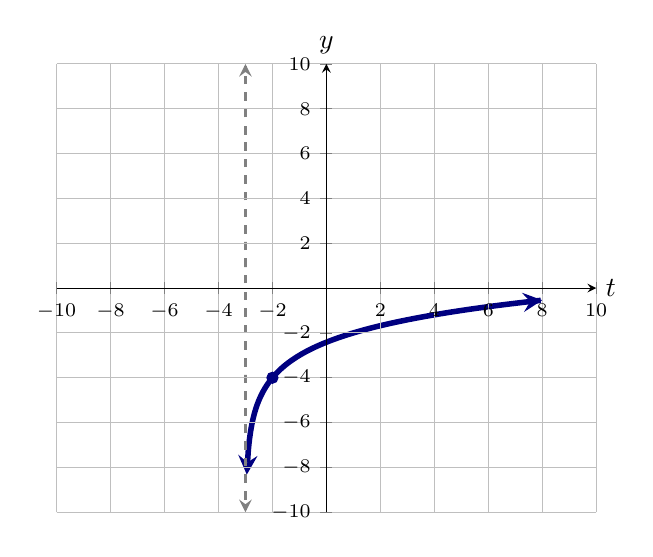
\begin{tikzpicture}
  \begin{axis}[
            domain=-10:10, ymax=10, xmax=10, ymin=-10, xmin=-10,
            axis lines =center, xlabel=$t$, ylabel=$y$, grid = major,
            ytick={-10,-8,-6,-4,-2,2,4,6,8,10},
            xtick={-10,-8,-6,-4,-2,2,4,6,8,10},
            ticklabel style={font=\scriptsize},
            every axis y label/.style={at=(current axis.above origin),anchor=south},
            every axis x label/.style={at=(current axis.right of origin),anchor=west},
            axis on top
          ]
          

			\addplot [line width=2, penColor, smooth,samples=200,domain=(-2.95:8),<->] {ln(x+3)/ln(2)-4};

			\addplot [line width=1, gray, dashed,samples=200,domain=(-10:10),<->] ({-3},{x});
            %\addplot [line width=1, gray, dashed,samples=200,domain=(-10:10),<->] ({x},{x});


			\addplot[color=penColor,fill=penColor,only marks,mark=*] coordinates{(-2,-4)};






           

  \end{axis}
\end{tikzpicture}
\end{image}




Our analysis tells us that:

\begin{itemize}
\item The implied domain of $M$ is $(-3,\infty)$.
\item The implied range of $M$ is $\mathbb{R}$.
\item $M$ is always \wordChoice{\choice[correct]{increasing} \choice{decreasing}}.
\item $M$ has no maximums or minimums.
\item $\lim\limits_{t \to -3^+} M(t) = -\infty$
\item $\lim\limits_{t \to \infty} M(t) = \infty$
\end{itemize}




We can also see that the graph will have a horizontal intercept, which means the function has a zero. \\


$M(t) = \log_2(t+3) - 4 = 0$ \\


\begin{align*}
\log_2(t+3) - 4 & = 0 \\
\log_2(t+3) & = 4 \\
2^{\log_2(t+3)} & = 2^{\answer{4}} \\
t+3 & = 16 \\
t & = 13
\end{align*}


$\blacktriangleright$ \textbf{Remember:} $\log_2(t+3)$ is the thing that you raise $2$ to, to get $t+3$ and $\log_2(t+3) = 4$.  Therefore, $4$ is the thing that you raise $2$ to, to get $t+3$. $t+3$ must be $16$.









\end{explanation}

\end{example}



$M(t)$ is a logarithmic function, so it must have a partner (shifted) exponential function.  The pairs for $M$ look like $(t, M(t))$ or just $(t,M)$. The pairs for the (shifted) exponential function would look like $(M, t)$.  The roles of $M$ and $t$ would be switched. $M$ would be the variable in the formula. $t$ would be the function value.


We can obtain the formula for this partner (shifted) exponential function by solving the logarithmic formula for $t$.



\begin{explanation}

\begin{align*}
\log_2(t+3) - 4 & = M \\
\log_2(t+3) & = M + 4 \\
2^{\log_2(t+3)} & = 2^{\answer{M+4}} \\
t+3 & = 2^{M+4} \\
t & = \answer{2^{M+4} - 3}
\end{align*}

\end{explanation}


$\blacktriangleright$ \textbf{Remember:} $\log_2(t+3)$ is the thing that you raise $2$ to, to get $t+3$ and $\log_2(t+3) = M+4$.  Therefore, $M+4$ is the thing that you raise $2$ to, to get $t+3$





Here is the graph of both the logarithmic and the associated exponential functions.





\begin{image}
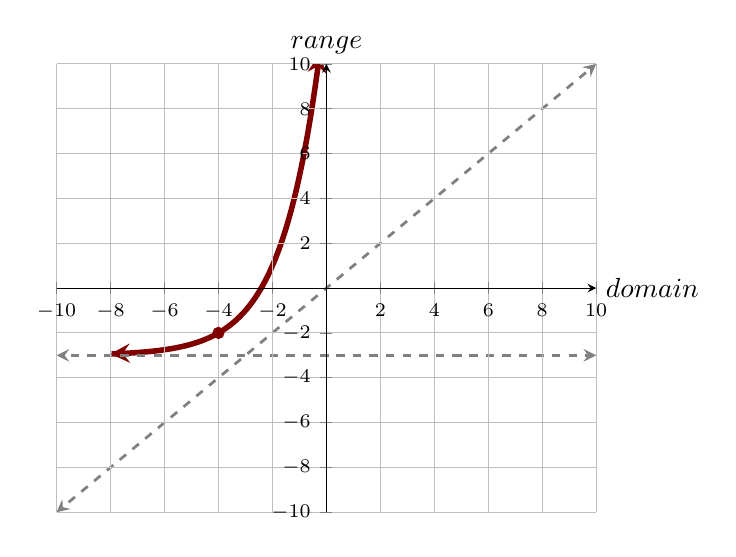
\begin{tikzpicture}
  \begin{axis}[
            domain=-10:10, ymax=10, xmax=10, ymin=-10, xmin=-10,
            axis lines =center, xlabel=$domain$, ylabel=$range$, grid = major,
            ytick={-10,-8,-6,-4,-2,2,4,6,8,10},
            xtick={-10,-8,-6,-4,-2,2,4,6,8,10},
            ticklabel style={font=\scriptsize},
            every axis y label/.style={at=(current axis.above origin),anchor=south},
            every axis x label/.style={at=(current axis.right of origin),anchor=west},
            axis on top
          ]
          

			%\addplot [line width=2, penColor, smooth,samples=200,domain=(-2.95:8),<->] {ln(x+3)/ln(2)-4};
			\addplot [line width=2, penColor2, smooth,samples=200,domain=(-8:-0.25),<->] {2^(x+4)-3};

			%\addplot [line width=1, gray, dashed,samples=200,domain=(-10:10),<->] ({-3},{x});
            \addplot [line width=1, gray, dashed,samples=200,domain=(-10:10),<->] ({x},{-3});
            \addplot [line width=1, gray, dashed,samples=200,domain=(-10:10),<->] ({x},{x});


			%\addplot[color=penColor,fill=penColor,only marks,mark=*] coordinates{(-2,-4)};
			\addplot[color=penColor2,fill=penColor2,only marks,mark=*] coordinates{(-4,-2)};






           

  \end{axis}
\end{tikzpicture}
\end{image}












\begin{image}
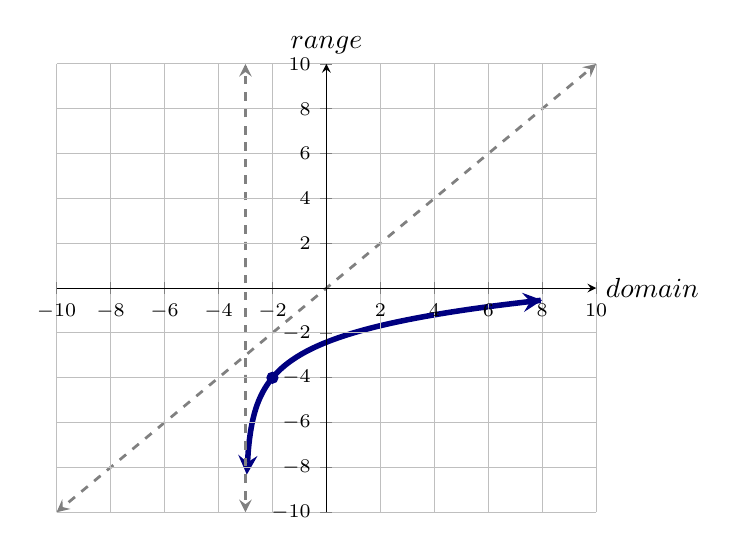
\begin{tikzpicture}
  \begin{axis}[
            domain=-10:10, ymax=10, xmax=10, ymin=-10, xmin=-10,
            axis lines =center, xlabel=$domain$, ylabel=$range$, grid = major,
            ytick={-10,-8,-6,-4,-2,2,4,6,8,10},
            xtick={-10,-8,-6,-4,-2,2,4,6,8,10},
            ticklabel style={font=\scriptsize},
            every axis y label/.style={at=(current axis.above origin),anchor=south},
            every axis x label/.style={at=(current axis.right of origin),anchor=west},
            axis on top
          ]
          

      \addplot [line width=2, penColor, smooth,samples=200,domain=(-2.95:8),<->] {ln(x+3)/ln(2)-4};
      %\addplot [line width=2, penColor2, smooth,samples=200,domain=(-8:-0.25),<->] {2^(x+4)-3};

      \addplot [line width=1, gray, dashed,samples=200,domain=(-10:10),<->] ({-3},{x});
            %\addplot [line width=1, gray, dashed,samples=200,domain=(-10:10),<->] ({x},{-3});
            \addplot [line width=1, gray, dashed,samples=200,domain=(-10:10),<->] ({x},{x});


      \addplot[color=penColor,fill=penColor,only marks,mark=*] coordinates{(-2,-4)};
      %\addplot[color=penColor2,fill=penColor,only marks,mark=*] coordinates{(-4,-2)};






           

  \end{axis}
\end{tikzpicture}
\end{image}













































\begin{example}  Logarithmic Function


\begin{explanation}

Analyze   $K(x) = -2 \, \log_3(4-x)$ \\


$\blacktriangleright$ The inside of the logarithm is $4-x$ and this equals $0$ when $x=\answer{4}$.  $x=4$ has to be the vertical asymptote.

$\blacktriangleright$ The inside of the logarithm is $4-x$, and this is positive for $x<4$.  The graph must move to the right.

$\blacktriangleright$ The leading coefficient is $-2$, which is \wordChoice{\choice{positive} \choice[correct]{negative}} .  Therefore, the graph is flipped vertically from the basic graph. It goes up the asymptote. 

$\blacktriangleright$ $4-x=1$ when $x=3$. Therefore, the anchor point $(1,0)$ has moved to $\left( \answer{3}, \answer{0} \right)$.





Graph of $y = K(x)$.

\begin{image}
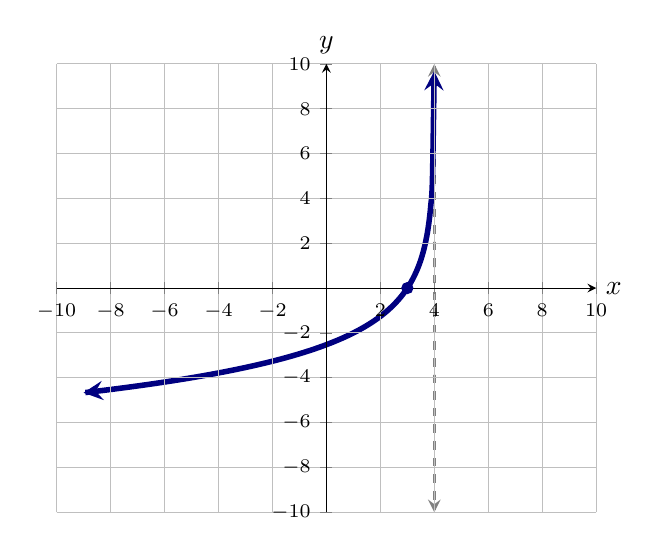
\begin{tikzpicture}
  \begin{axis}[
            domain=-10:10, ymax=10, xmax=10, ymin=-10, xmin=-10,
            axis lines =center, xlabel=$x$, ylabel=$y$, grid = major,
            ytick={-10,-8,-6,-4,-2,2,4,6,8,10},
            xtick={-10,-8,-6,-4,-2,2,4,6,8,10},
            ticklabel style={font=\scriptsize},
            every axis y label/.style={at=(current axis.above origin),anchor=south},
            every axis x label/.style={at=(current axis.right of origin),anchor=west},
            axis on top
          ]
          

			\addplot [line width=1, gray, dashed,samples=200,domain=(-10:10),<->] ({4},{x});

      \addplot [line width=2, penColor, smooth,samples=200,domain=(-9:3.995),<->] {-2*ln(4-x)/ln(3)};

			
            %\addplot [line width=1, gray, dashed,samples=200,domain=(-10:10),<->] ({x},{x});


			\addplot[color=penColor,fill=penColor,only marks,mark=*] coordinates{(3,0)};






           

  \end{axis}
\end{tikzpicture}
\end{image}









\begin{itemize}
\item The natural or implied domain of $K$ is $(-\infty, 4)$.
\item The implied range of $K$ is $\mathbb{R}$.
\item $K$ is always increasing.
\item $K$ has no maximums or minimums.
\item $\lim\limits_{x \to 4^-} K(x) = \infty$
\item $\lim\limits_{x \to -\infty} K(x) = -\infty$
\end{itemize}




\end{explanation}
\end{example}









Reversing all of the pairs will give the associated exponential function.  \\



$K(x)$ is a logarithmic function, so it must have a partner exponential function.  The pairs for $K$ look like $(x, K)$. The pairs for the exponential function would look like $(K, x)$.  The roles of $K$ and $x$ would be switched. $K$ would be the variable in the exponential formula. $x$ would be the exponential function value.


We can obtain the formula for this partner exponential function by solving the logarithmic formula for $x$.



\begin{explanation}

\begin{align*}
-2 \,\log_3(4-x) & = M \\
\log_3(4-x) & = \answer{-\frac{M}{2}} \\
3^{\log_3(4-x)} & = \answer{3}^{-\frac{M}{2}} \\
4 - x & = 3^{-\frac{M}{2}} \\
\answer{4 - 3^{-\frac{M}{2}}} & = x \\
\end{align*}

\end{explanation}




$\blacktriangleright$ \textbf{Remember:} $\log_3(4-x)$ is the thing that you raise $3$ to, to get $4-x$ and $\log_3(4-x) = - \frac{M}{2}$.  Therefore, $- \frac{M}{2}$ is the thing that you raise $3$ to, to get $4-x$





Here is the graphs of both the logarithmic and the associated exponential functions.





\begin{image}
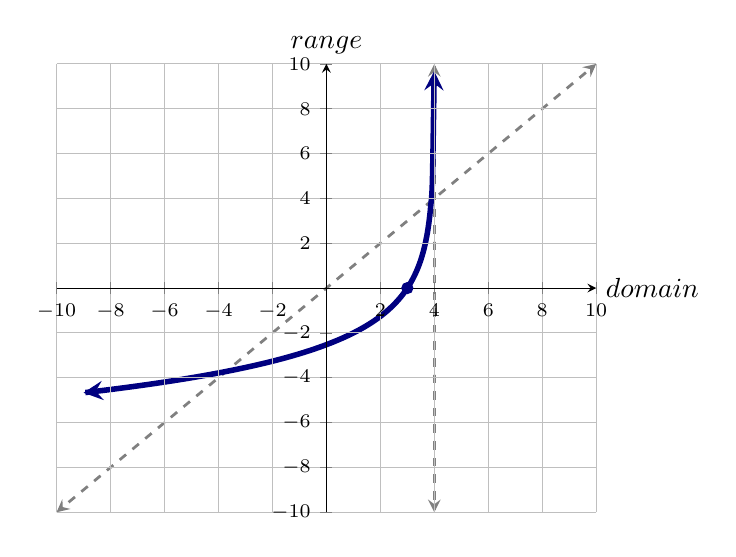
\begin{tikzpicture}
  \begin{axis}[
            domain=-10:10, ymax=10, xmax=10, ymin=-10, xmin=-10,
            axis lines =center, xlabel=$domain$, ylabel=$range$, grid = major,
            ytick={-10,-8,-6,-4,-2,2,4,6,8,10},
            xtick={-10,-8,-6,-4,-2,2,4,6,8,10},
            ticklabel style={font=\scriptsize},
            every axis y label/.style={at=(current axis.above origin),anchor=south},
            every axis x label/.style={at=(current axis.right of origin),anchor=west},
            axis on top
          ]
          
			\addplot [line width=1, gray, dashed,samples=200,domain=(-10:10),<->] ({4},{x});

      \addplot [line width=1, gray, dashed,samples=200,domain=(-10:10),<->] ({x},{x});

      \addplot [line width=2, penColor, smooth,samples=200,domain=(-9:3.995),<->] {-2*ln(4-x)/ln(3)};

			

			\addplot[color=penColor,fill=penColor,only marks,mark=*] coordinates{(3,0)};


			



           

  \end{axis}
\end{tikzpicture}
\end{image}

















\begin{image}
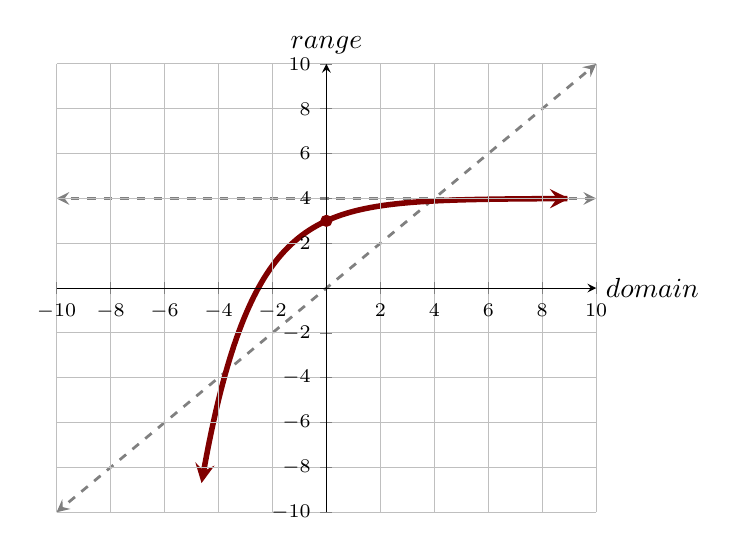
\begin{tikzpicture}
  \begin{axis}[
            domain=-10:10, ymax=10, xmax=10, ymin=-10, xmin=-10,
            axis lines =center, xlabel=$domain$, ylabel=$range$, grid = major,
            ytick={-10,-8,-6,-4,-2,2,4,6,8,10},
            xtick={-10,-8,-6,-4,-2,2,4,6,8,10},
            ticklabel style={font=\scriptsize},
            every axis y label/.style={at=(current axis.above origin),anchor=south},
            every axis x label/.style={at=(current axis.right of origin),anchor=west},
            axis on top
          ]
          
      


      \addplot [line width=1, gray, dashed,samples=200,domain=(-10:10),<->] ({x},{4});

      \addplot [line width=1, gray, dashed,samples=200,domain=(-10:10),<->] ({x},{x});


      \addplot [line width=2, penColor2, smooth,samples=200,domain=(-4.627:9),<->] {4-3^(-x/2)};

      

      \addplot[color=penColor2,fill=penColor2,only marks,mark=*] coordinates{(0,3)};

      


           

  \end{axis}
\end{tikzpicture}
\end{image}












\begin{center}
\textbf{\textcolor{green!50!black}{ooooo=-=-=-=-=-=-=-=-=-=-=-=-=ooOoo=-=-=-=-=-=-=-=-=-=-=-=-=ooooo}} \\

more examples can be found by following this link\\ \link[More Examples of Percent Change]{https://ximera.osu.edu/csccmathematics/precalculus1/precalculus1/percentChange/examples/exampleList}

\end{center}



\end{document}
